\begin{multicols}{3}
\subsection{Basic Semiconductor Physics}
%\begin{tabularx}{\linewidth}{l X}
\begin{tabular}{p{5.5cm}p{2.75cm}}
$ v_{th}= \sqrt{\frac{3kT}{m^\ast}} $ & Thermal velocity  \\ %of a particle \\
$ E= \frac{hc}{\lambda} $ & Energy of photon \\ %Energy of a mass-less particle (photon) \\
$p=\sqrt{2mE}; \ p=\frac{h}{\lambda}; \ \lambda=\frac{h}{\sqrt{2mE}}$ & Momentum, wavelength \\
$\tau=\frac{m_e \mu_e}{q}$ & Mean free time \\
$\frac{k_BT}{q}=0.025875 \ \text{eV} \approx 0.026 \ \text{eV}$ & \\
Donors: Group 5- P As, Sb & Doping elements \\
Acceptors Group 3- B, Al, Ga, In
\end{tabular}
%\end{tabularx} 
\subsection{FERMI Levels}
\begin{tabular}{p{4.25cm}p{4cm}}
$f(E)=\frac{1}{1+e^{(E-E_f)/k_BT}}$ 
$f(E)=(1+e^{(E-E_f)/k_BT})^{-1}$
$f(E) \approx e^{(E-E_f)/k_BT}$
& Fermi-Dirac Distribution Function: probability of finding an Electron at energy level E \\
$1-f(E)$ & Probability of finding a hole at energy level E \\
$E_f-E_i=k_BT\left[\ln \left(\frac{n}{n_i} \right)\right]$ & Fermi level of N-Type (when $N_D \gg N_A$) 
\\
To convert J to eV & $6.2415 \times 10^{18} \text{eV/J}$ \\
$E_i-E_f=k_BT\left[\ln \left(\frac{p}{n_i} \right)\right]$ & Fermi level of P-Type (when $N_A \gg N_D$) \\
$q\Phi_S = \chi [0.56-(E_f-E_i)]$ & Work function of silicon $\chi$: Electron affinity (4.05 eV) %(Units are eV)
\end{tabular}
\subsection{Semiconductor properties}

\begin{minipage}[h]{0.5\linewidth}
\textbf{N-Type}
\begin{enumerate}
\item[---] Dopant contributes extra electrons (donors) to increase conductivity.
\item[---] Electrons are majority carriers
\item[---] Holes are minority carriers
\item[---] Dopant are from Group 5 of periodic table: P, As, Sb
\end{enumerate}
\end{minipage}
\begin{minipage}[h]{0.5\linewidth}
\textbf{P-Type}
\begin{enumerate}
\item[---] Dopant accept extra holes (acceptor) to increase conductivity.
\item[---] Holes are majority carriers
\item[---] Electrons are minority carriers
\item[---] Dopant are from Group 3 of periodic table: B, Al, Ga, In
\end{enumerate}
\end{minipage}
\subsection{Built-in Potentials and Depletion Width}
%\vspace*{-1cm}
\begin{align*}
& V_{bi}=\frac{kT}{q} \ln \left[\frac{n_n}{n_p}\right]=\frac{kT}{q} \ln \left[ \frac{N_d N_a}{n_i^2}\right] \\
& V_{bi} = 0.56 + \frac{kT}{q} \ln \left[\frac{N_d}{n_i}\right] \ (p^+n \text{junction}) \\
& V_{bi} = 0.56 + \frac{kT}{q} \ln \left[\frac{N_a}{n_i}\right] \ (pn^+ \text{junction}) \\
& V_{bi}=V_n-V_p
\end{align*}
$\displaystyle E_x = \frac{v_d}{\mu_e}$ Electric field / velocity-mobility relationship

\hfill Note that $K_s \epsilon_0=1.045 \times 10^{-12} \ \frac{\text{F}}{\text{cm}}$ for Silicon.
\begin{align*}
& x_n=\left\{ \frac{2K_s \epsilon_0}{q} V_{bi} \left[\frac{N_a}{N_d(N_a+N_d)}\right] \right\}^{1/2} \\
& x_p=\left\{ \frac{2K_s \epsilon_0}{q} V_{bi} \left[\frac{N_d}{N_a(N_a+N_d)}\right] \right\}^{1/2} \\
& x_d = \left\{ \frac{2K_s \epsilon_0}{q} V_{bi} \left[\frac{1}{N_a}+\frac{1}{N_d}\right] \right\}^{1/2} \\
& x_p=\left(\frac{N-d}{N_a}\right)x_n; \ x_n = \left(\frac{N_a}{N_d}\right)x_p \\
& x_d = x_n + x_p
\end{align*}
%Example: Total Charge in N-side of PN junction: Total charge in a n region consists of 1) Excess minority holes and 2) The fixed positive charge in the depletion layer.

\begin{align*}
& Q_p=Aq\frac{1}{2}W^\prime_BP^\prime_n(x_n) \\
& \ \ = Aq\frac{1}{2}W^\prime_B p_{n0}(x_n) \left[e^{\frac{qV_a}{kT}-1}\right] \\
& Q_{SC} = Aq N_d x_n \\
& Q_{n-side}=Q_p+Q_{sc} \quad E_{max}=\frac{2(V_{bi}-V_a)}{x_d}
\end{align*}
\begin{tabular}{p{5cm}p{3.25cm}}
$n^\prime_p(-x_p)=n_{p0}(-x_p)\left[e^{\frac{qV_a}{kT}}-1\right]$ & Excess minority \hfill \break carrier density \\
$p^\prime_n(-x_p)=p_{n0}(x_n)\left[e^{\frac{qV_a}{kT}}-1\right]$ & $n^\prime_p$ \# of holes n-side \\
$n^\prime \equiv n - n_0$ $n_{p0}=\frac{n_i^2}{N_a}$ 
$p_{n0}=\frac{n_i^2}{N_d}$ therm equil mino carr & $n_0$ thermal equili \hfill \break carrier concent \\
\end{tabular}
$C_j=  A\left[\cfrac{0.5q \epsilon_0}{\left(\frac{1}{N_a}+\frac{1}{N_d}\right)(V_{bi}-V_a)}\right]^{1/2}$ \hfill \break
note: for zero-bias junction capacitance, use first(above) equation with
$V_a= 0$ \hfill \break
 $C_j=\frac{K_s \epsilon_0}{x_d} $ $C_j= \frac{q}{kT} \left(\frac{qL_pp_{n0}}{2}+\frac{qL_nn_{p0]}}{2}\right)$

\subsection{CARRIER CONCENTRATION}
\begin{tabular}{p{5.25cm}p{3cm}}
$n_i= \sqrt{N_c N_v}\exp(-E_G/2k_BT)$ $n=p$ & Intrinsic carrier concentration \\
$np=n_i^2; \ n=\frac{n_i^2}{N_D}; \ p=\frac{n_i^2}{N_A}$ & Product of electron and hole CONC \\
$n=n_ie^{(E_f-E_i)/k_BT}$ \hfill \newline $n=\frac{N_d-N_a}{2}+\left[ \left(\frac{N_d-N_a}{2} \right)^2+n_i^2\right]^{1/2}$ & Electron concentration (when $N_a$ is close to $N_d$ --- 1 order of mag \\
$p=n_ie^{(E_f-E_i)/k_BT}$ \hfill \newline $p=\frac{N_a-N_d}{2}+\left[ \left(\frac{N_a-N_d}{2} \right)^2+n_i^2\right]^{1/2}$ & Hole Concentration ($N_d$ close to $N_a$) \\
$n \cong N_d-N_a, \ p \cong N_a - N_d $ \hfill \newline
% Add in current density to converse space lol
Current Density and Electron current density (similar for hole current density) \hfill \newline
$J_x=(nq\mu_n+pq\mu_p)E_x$ \hfill \newline
$J_n=q \mu_n nE_x+qD_n\frac{dn}{dx}$ \hfill \newline 
& Electron \& Hole Conc for N and P-type SC (when $N_d \gg N_a$ or $N_a \gg N_d$ $>$ one order of mag) \\
$D_n=\frac{k_BT}{q}\mu_n; \ D_p=\frac{k_BT}{q}\mu_p$ & Diffusion coefficient \\
$L_n=\sqrt{D_n \tau_n}; \ L_p=\sqrt{D_p \tau_p}$ & Minority carrier diffusion length \\
$\rho = \frac{1}{q(\mu_n n + \mu_p)}$ & Resistivity (conductivity is $\rho^{-1}$ \\
$\rho_n=\frac{1}{q \mu_n N_d}; \ \rho_p=\frac{1}{q \mu_p N_a}$ & Resistivity for n \& p \\
$\bar{v_n}= \mu_n E$ & Velocity of propagation of $e^-$ with applied bias $E$ \\
$V_H=\frac{-I_xB_z}{qnt}$ & Hall voltage (p-type no negative sign) \\
$\sigma=\frac{GL}{A_{CS}}=\frac{L}{RA_{CS}}$ & Conductivity of a material \\
$\mu_n=\frac{\sigma}{qn}; \ \mu_p=\frac{\sigma}{qp}$ & Electron and hole mobility
\end{tabular}
\subsection{Current Density}
$N_a \gg N_d$: P-type $\rightarrow$ Calculate $L_p$ \hfill \break
$N_d \gg N_a$: N-type $\rightarrow$ Calculate $L_n$ \hfill \break
Determination of long-short base diode
(Note: W may be given as wafer thickness) $W=\frac{2\epsilon_s V_{bi	}}{q} \left[\frac{N_a+N_d}{N_aN_d}
\right]^{12}$ 

$L < W:$, $(x_B \ \&  \ x_E) \ll  \ W_B \ \& \ W_E $ Short base diode \hfill \break
$L > W:$, $(x_B \ \&  \ x_E)  \gg\ W_B \ \& \ W_E $ Long base diode % \hfill \break

\textbf{Long base diode} \hfill \break 
$I=qAn_i^2 \left[\frac{D_p}{L_p N_d}+\frac{D_n}{L_n N_a}\right] \left(e^{\frac{qV_a}{k_BT}}-1 \right)$ \hfill \break 

\textbf{Short base diode} \hfill \break 
$I=qAn_i^2 \left[\frac{D_p}{W^\prime N_d}+\frac{D_n}{W_E^\prime N_a}\right] \left(e^{\frac{qV_a}{k_BT}-1} \right)$ \hfill \break 
Reserve saturation current due to electrons. \hfill \break
$I_{r(e)}=qA\left(\frac{D_p}{L_p}\right)p_n; p_n=\frac{n_i^2}{N_d}$

Reserve saturation current due to holes. \hfill \break
$I_{r(p)}=qA\left(\frac{D_n}{L_n}\right)p_p; p_p=\frac{n_i^2}{N_a}$
Total reverse saturation \hfill \break 
$I_r=I_{r(e)}+T_{r(p)}$
\subsection{Hall Effect}
\textbf{Type of semiconductor wafer} \hfill \break
$V_H < 0:$ N-Type \hfill \break
$V_H > 0:$ P-Type \hfill \break
Hall voltage(similar to p-type) \hfill \break
$V_H=\frac{-I_xB_z}{qnt}$ \hfill \break
$E_H=R_HJ_xB_x$ Hall effect field \hfill \break
$R_H=\frac{-1}{qn}; \ R_H=\frac{1}{qn}$ Hall coefficient \hfill \break
Majority Carrier Concentration \hfill \break
1. Find $R_H$ using Hall effect field equations \hfill \break
2. Find n using Hall coefficient equation.

\textbf{Assignment Solutions and Examples} \hfill \break
	\textbf{A silicon sample is doped with} $3\times10^{17} cm^{-3}$ \textbf{phosphorus atoms and} $7\times 10^{17} \ cm^{-3}$ \textbf{arsenic atoms. Find the thermal equilibrium carrier concentrations, majority carrier mobility, resistivity and location of the Fermi level for this sample. Sketch the thermal equilibrium band edge diagram}.

Arsenic and Phosphorous are donors, n-type semiconductors, $7 \times 10^{17} \ \si{c \meter}$ and $3\times 10^{17}  \si{c \meter}$.

\begin{align*}
& N_d = 7 \times 10^{17} \ \si{c \meter}^{-3} + 3\times 10^{17}  \si{c \meter}^{-3} = 1\times 10^{18} \ \si{c \meter}^{-3} \\
& n = \frac{N_d-N_a}{2}+\left[ \left(\frac{N_d-N_a}{2} \right)^2 + n_i^2 \right]^{1/2}= 1 \times 10^{18} \si{c \meter}^{-3}\\
& , \quad N_d >> n_i \quad \text{electron mobility: } \mu_n = \frac{q \tau}{m_n}
\end{align*}

Using Figure 2-5 for $10^{17}$, the carrier concentration is about $250 \ \si{c \meter}^2 / V-s$.

\begin{align*}
& \rho_n=\frac{1}{q \mu_n N_d}= \frac{1}{1.6 \ 10^{-19}250 \ 10^{18}} = 2.232 \times 10^{-2}\frac{\Omega}{\text{m}} \ 
 \end{align*}
The resistivity is $\rho_n = 2.232143 \times  10^{-4} \si{\ohm} \si{\meter}$.

%\vspace{-1.5cm}
\begin{align*}
& E_F - E_i = 0.026 \ln \left(\frac{1 \times 10^{18}}{1.5 \times 10^{10}} \right) = 0.468395 \ eV
\end{align*}
%\vspace{-1cm}
\textbf{Explain why tunneling is large in heavily doped metal-semiconductor contacts.} The narrow depletion width in the semiconductor results in a small barrier width for tunneling. Since tunneling increases exponentially with decreasing barrier width, it becomes very large in this case. \hfill \linebreak

\textbf{An extrinsic semiconductor bar is used in a Hall effect experiment. Can the data obtained be used to calculate the mobility of electrons and holes in the samples?} NO \hfill \break

\textbf{Introducing defects into a p-n diode allows it to switch faster.} TRUE

\textbf{Find the thermal equilibrium carrier concentrations for a silicon sample doped with} $3 \times 10^{17} \ \text{cm}^{-3}$ phosphorus atoms and $3 \times 10^{17} \ \text{cm}^{-3}$. Sketch the thermal equilibrium band edge diagram and find the position of the Fermi level. What is the maximum drift current density that can flow through this sample?

$n \approx N_d = 3 \times 10^{17} \ \text{cm}^{-3}= 6 \times 10^{17} \ \text{cm}^{-3}$
$p=\frac{n_i^2}{n}=\frac{2.25 \times 10^{20}}{6 \times 10^{12}}= 375 \ \text{cm}^{-3}$
$n=n_i \exp\left( \frac{E_f-E_i}{k_BT}\right)$ \hfill \linebreak
$E_f-E_i=k_B T \ln \left( \frac{n}{n_i} \right)=0.455 \ \text{eV}$ \hfill \break
Ignoring holes
$J=qnv$
$J_{max}=qnv_{sat} \rightarrow J_{max}=10^{6} \ \text{A/cm}^2$

A silicon p-n diode is formed by diffusing a high concentration of phosphorus into a 75 micron thick boron-doped wafer having a resistivity of 5 $\Omega-\text{cm}$ and minority carrier lifetime of $5 \mu$s. The junfction is formed $10 \ \mu$m below the surface with area $10^{-4} \ \text{cm}^2$. Find in built-in potential. Calculate the current flowing through the diode under and applied forward bias of 0.5 volts. Sketch the excess minority carrier distribution at steady state and at $t=t_s$ if $\delta=0.2$

$V_{bi}=\frac{k_BT}{q} \ln \left(\frac{N_a}{n_i}\right)+0.56 V$
Using the chart from Vol.I(p.71) $V_{bi}=0.877 V $ \hfill \linebreak
$L_n=\sqrt{D_n \tau_n} = 130 \mu \text{m}$, $L_n >65 \mu \text{m} $ $I=Aqn_i^2 \left(\frac{D_p}{N_dW_0^\prime}+\frac{D_n}{N_aW_E^\prime} \right) (e^{qV_a/k_BT}-1)=1.4 \mu \text{A}$ if $\delta = 0.2 $ at $t=t_s $, then 20 \% of the carriers have been removed during the storage time. \hfill \linebreak

\textbf{Calculate the energy of an electron in the ground state of an infinite quantum well if it has a wavelength of 5 nm}.
if $\lambda=5 \text{nm} \rightarrow L=2.5 \text{nm}$ and $E_q=\frac{\hbar^2 \pi^2}{2mL^2} = 60 \ \text{meV}$ \hfill \break

\textbf{When using the resistivity value of a semiconductor to find its doping level via a graph such as on p.71 of Vol.I, what implicit assumption is being made.}
Only one dopant type is present, i.e, the semiconductor is not compensated. \hfill \break

\textbf{Show that the turn-on time for a long base p-n junction diode is given by the minority carrier lifetime by explicitly solving for the ratio} $Q_P(\infty)/I_F$.

$Q_P(\infty)= qA \int_{x_n}^{\infty}p_{n0} \left(e^{qV_a/k_BT} -1 \right) \exp \left(- \frac{x-x_n}{L_p}\right) \ dx$
$=q\frac{An_i^2}{N_d} \left( e^{\frac{qV_{bi}}{k_BT}}-1 \right)L_p$
$I_F=qAn_i^2\frac{D_p}{N_dL_p} \left(e^{\frac{qV_{bi}}{k_BT}}-1 \right)$ and $\frac{Q_p(\infty)}{I_F}=\frac{L_p^2}{D_p}=\tau_p$ \hfill \break

\textbf{If an ideal metal-semiconductor junction is made between n-type silicon and aluminum} ($q\Phi_M=4.1$ eV) what must the doping level be in order for the built-in potential to be zero in thermal equilibrium?

$\Phi_i=\Phi_M-\Phi_s=0 \rightarrow$ $q\Phi_s=4.1$ eV $=qX+E_i-E_f$
$E_i-E_f=0.05$ eV and $E_f-E_i=0.51$ eV $\rightarrow n \approx N_d=n_i \exp \left(\frac{E_f-E_i}{k_BT} \right)=4.75 \times 10^{18} \ \text{cm}^{-3}$ \hfill \break 

\textbf{An abrupt lose-base silicon pn junction diode has} $N_d=5 \times 10^{16} \ \text{cm}^{-3}$, $N_a=8 \times 10^{17} \ \text{cm}^{-3}$ and a cross-sectional area of $2\times 10^{-1} \ \text{cm}^{-2}$. \textbf{Calculate the built-in potential for this junction and sketch the thermal equilibrium band edge diagram.} If $\tau_p=\tau_n=0.5 \mu$s calculate the current flowing through the junction if it is subjected to 0.75 V applied forward bias.

$V_{bi}=\frac{k_BT}{q} \ln \frac{N_dN_a}{n_i^2}=0.853 \ V$ $I=A_0 q n_i^2 \left(\frac{D_p}{N_dL_p}+\frac{D_n}{N_aL_n}\right) \left(e^{qV_a/k_BT}-1 \right)$
From the given doping levels we can lock up that $D_p=9.5 \ \text{cm}^2\text{s}^{-1}$ and $D_n=8 \ \text{cm}^2 \text{s}^{-1}$
$L_p=\sqrt{D_p \tau_p}=21.8 \mu$m and $L_n=\sqrt{D_n \tau_n}=20 \mu$m $I=2.236 \ \text{mA}$
%\end{multicols}
%   \begin{multicols}{3}
  \medbreak\noindent\minipage{\columnwidth}
            %\centering % if smaller than \columnwidth
            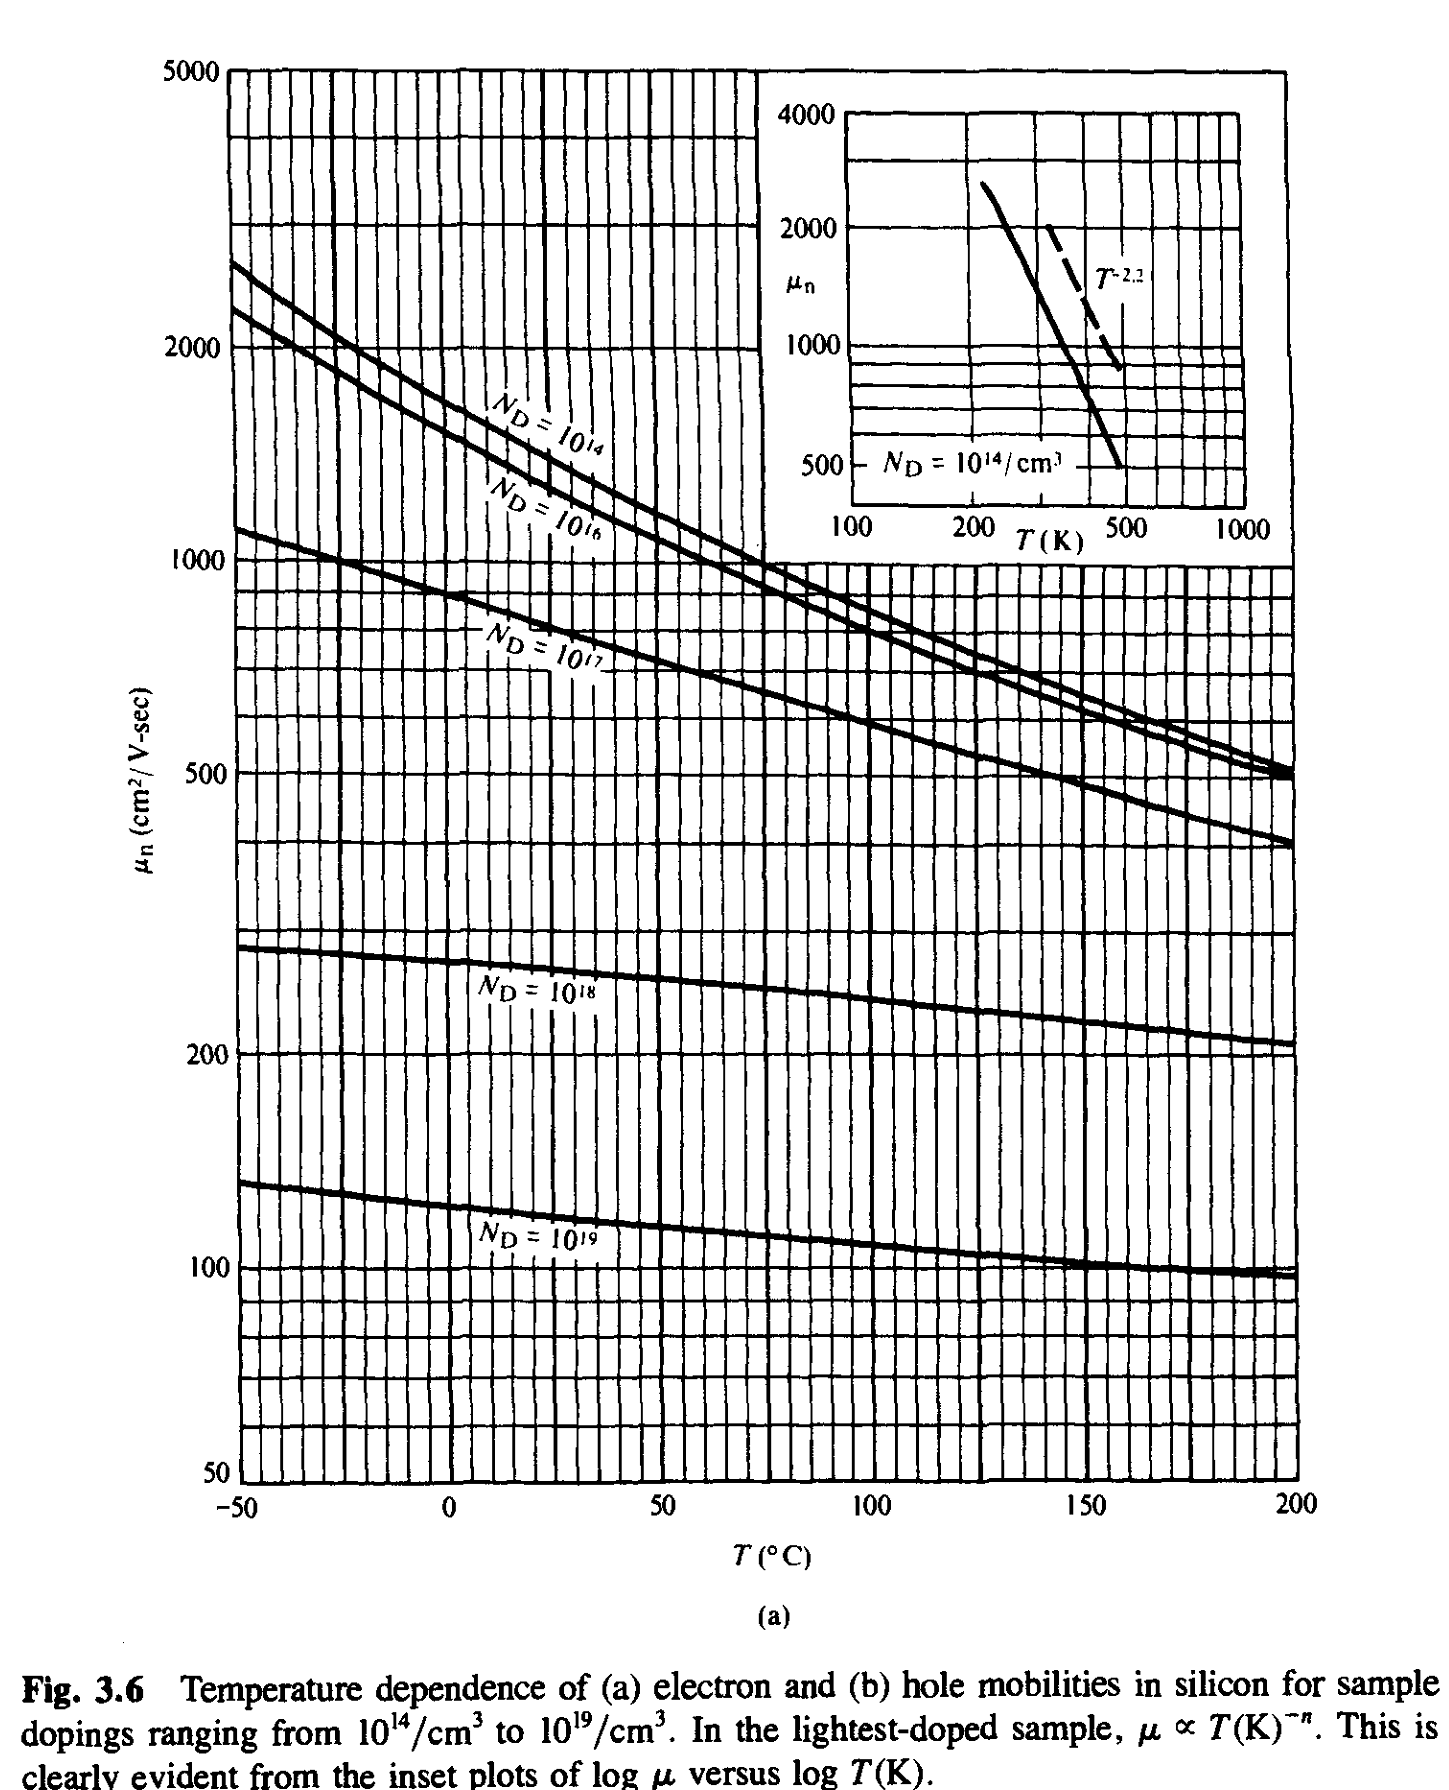
\includegraphics[width=\columnwidth]{V1Figure3-6.png}
            %\captionof{figure}{some caption} % optional
            %\captionof{figure}{some caption} % optional
        \endminipage\medbreak

A silicon p-n diode is formed by diffusing a high concentration of boron atoms into a $500 \mu$ m thick n-type wafer having a resistivity $\rho = 1 \Omega -$cm. The p-n junction has an area of $10^{-4}$ \ $\text{cm}^2$ and can be considered to be a step junction. Assume $\tau_e=\tau_h=1 \mu$s. Calculate the built-in potential, $V_0$ (do not assume a value for $N_a$). Calculate the current flowing through the diode under 0.6 V forward bias using ideal diode theory.

$V_o=\frac{k_BT}{q} \ln(\frac{N_dN_a}{N_a^2})=0.026 \ln(\frac{5 \times 10^{15}}{1.5 \times 10^{10}})+\frac{k_BT}{q}+\ln(\frac{N_a}{N_i})$. $N_a$ is very large $E_f$ will be very close to $E_v$, the valence band edge on the p-side: $V_o=0.33 V+ \frac{0.5E_g}{q}=0.33+0.56 V=0.89 V$ \hfill \break
From chart $D_{h(n-side)}=12 \ \text{cm}^2 \text{s}^{-1} \rightarrow L_h=\sqrt{D_h \tau_h}=34.6 \ \mu$m

$I=Aqn_i^2 \left(\frac{D_h}{N_dL_h}+\frac{D_e}{N_aL_e}\right)(e^{\frac{qV_a}{k_BT}}-1)$
$I=27 \ \mu$A.
%\vspace*{-1cm}
          \medbreak\noindent\minipage{\columnwidth}
            %\centering % if smaller than \columnwidth
            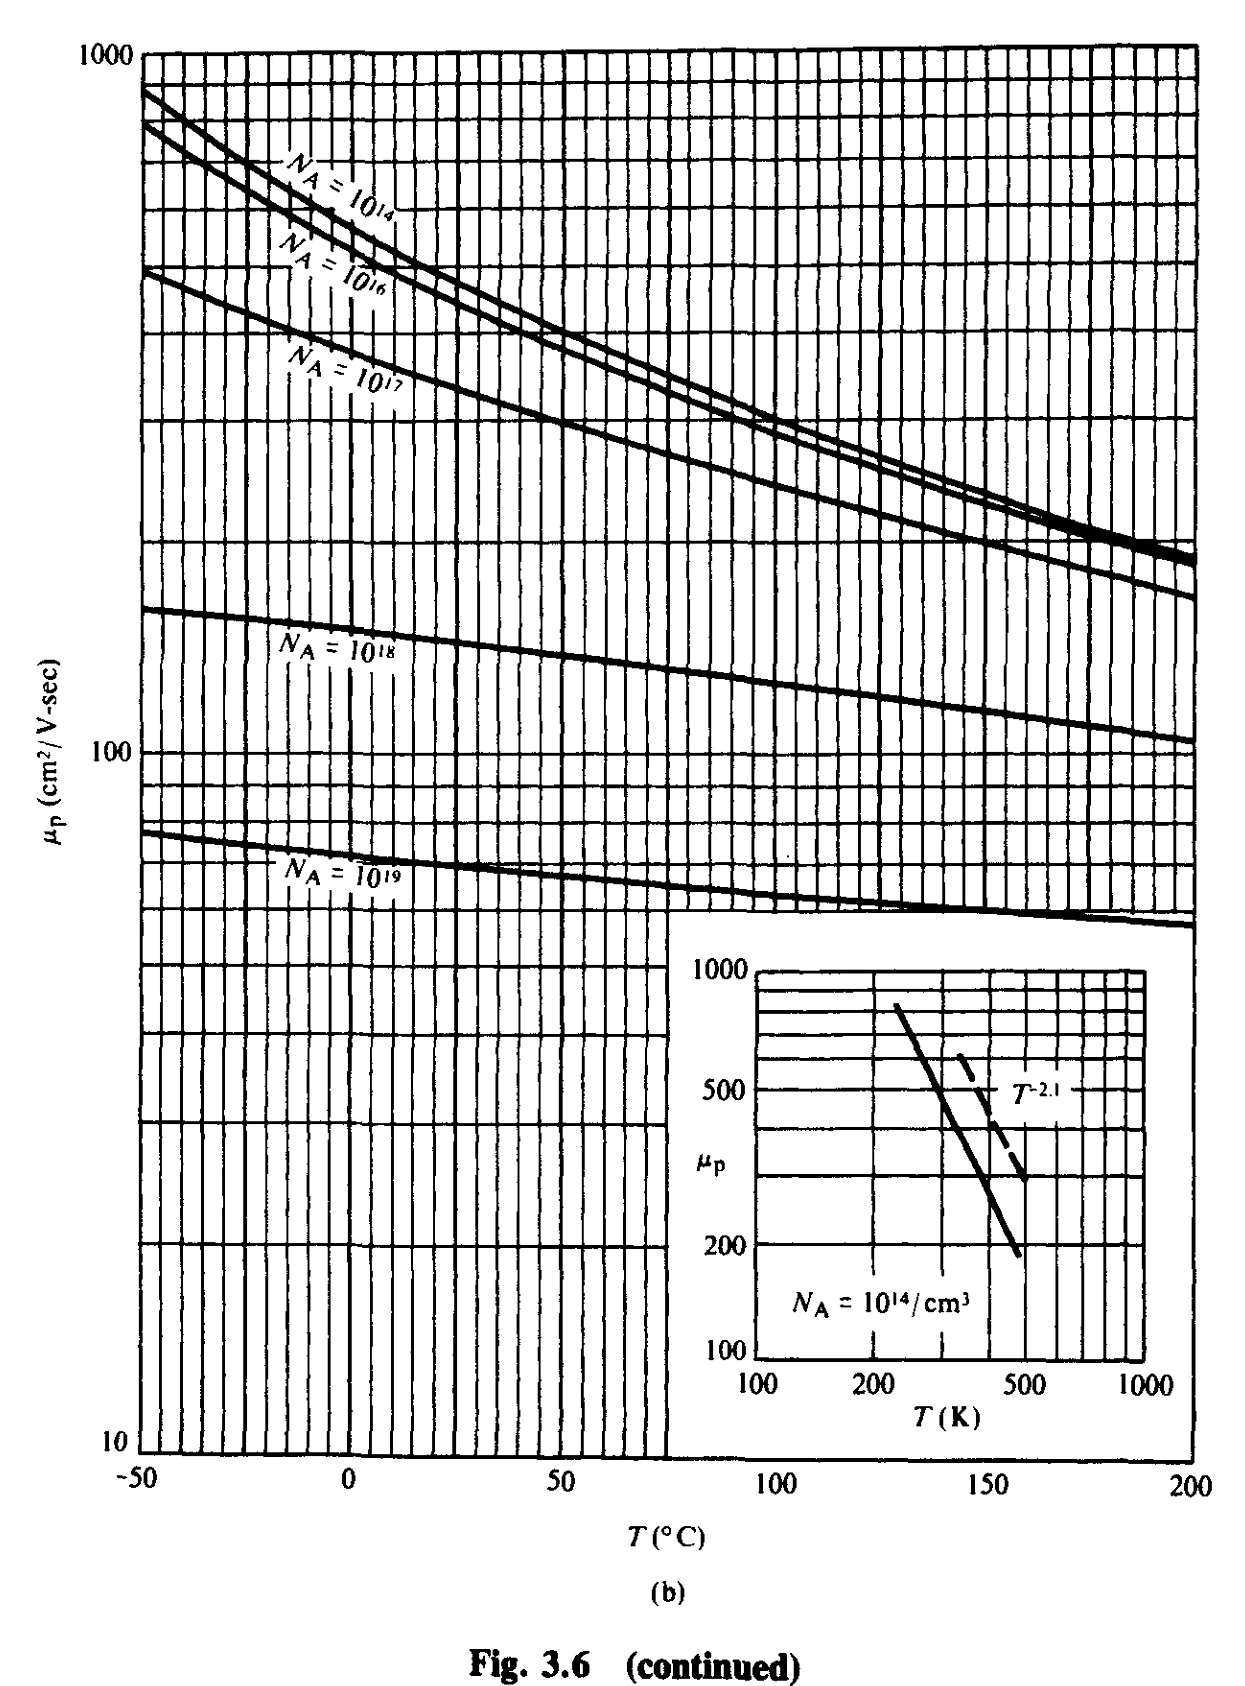
\includegraphics[width=\columnwidth]{V1Figure3-6b.png}
            %\captionof{figure}{some caption} % optional
            %\captionof{figure}{some caption} % optional
        \endminipage\medbreak 
        \textbf{An ideal p-n junction with cross-section } $A=5\times 10^{-5} \text{cm}^2$ \textbf{is made from silicon regions doped } $2\times 10^{18} \text{cm}^{-3}$ p-type and $10^{17}$ n-type with neutral region widths of $35 \mu$m and $10 \mu$m, respectively. \textbf{What is the value of the built-in voltage} If $\tau_n=\tau_p=0.5 \mu$s, calculate the current flowing through the junction under an applied bias of 0.5 V.
        $V_{bi}=\frac{k_B}{q} \ln \left(\frac{N_d N_a}{n_i^2}\right)=0.895 V$
        Fig.3.5 Vol I: $\mu_p=330 \frac{\text{cm}^2}{\text{Vs}} $ 
        $\rightarrow D_P=8.58 \ \frac{\text{cm}^2}{\text{s}}$
        and $L_p=\sqrt{D_p \tau_p}=20.7 \ \mu$m. 
        
        $\mu_n=190 \frac{\text{cm}^2}{\text{Vs}} $ 
        $\rightarrow D_n=4.94 \ \frac{\text{cm}^2}{\text{s}}$
        and $L_n=\sqrt{D_n \tau_p}=15.7 \ \mu$m. Therefore the diode is short on the n-side and long on the p-side. The current in this case is given by
        $I=Aqn_i^2 \left(\frac{D_p}{N_dx_B}+\frac{D_n}{N_a L_n}\right)(e^{\frac{qV_a}{k_BT}}-1)$
        \medbreak\noindent\minipage{\columnwidth}
            %\centering % if smaller than \columnwidth
            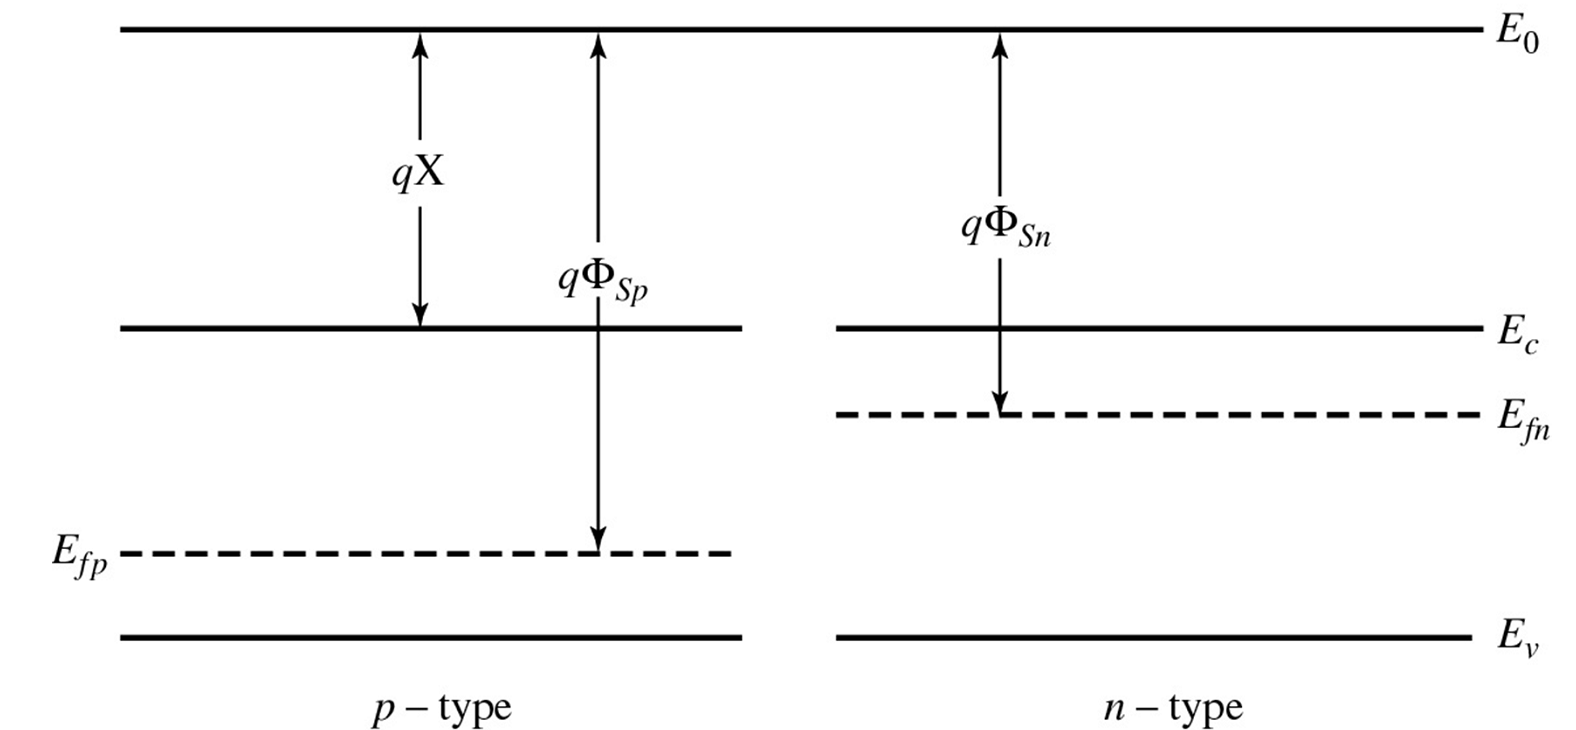
\includegraphics[width=\columnwidth]{LectureNotesIIJunc.png}
            %\captionof{figure}{some caption} % optional
            %\captionof{figure}{some caption} % optional
        \endminipage\medbreak   
          \medbreak\noindent\minipage{\columnwidth}
            %\centering % if smaller than \columnwidth
            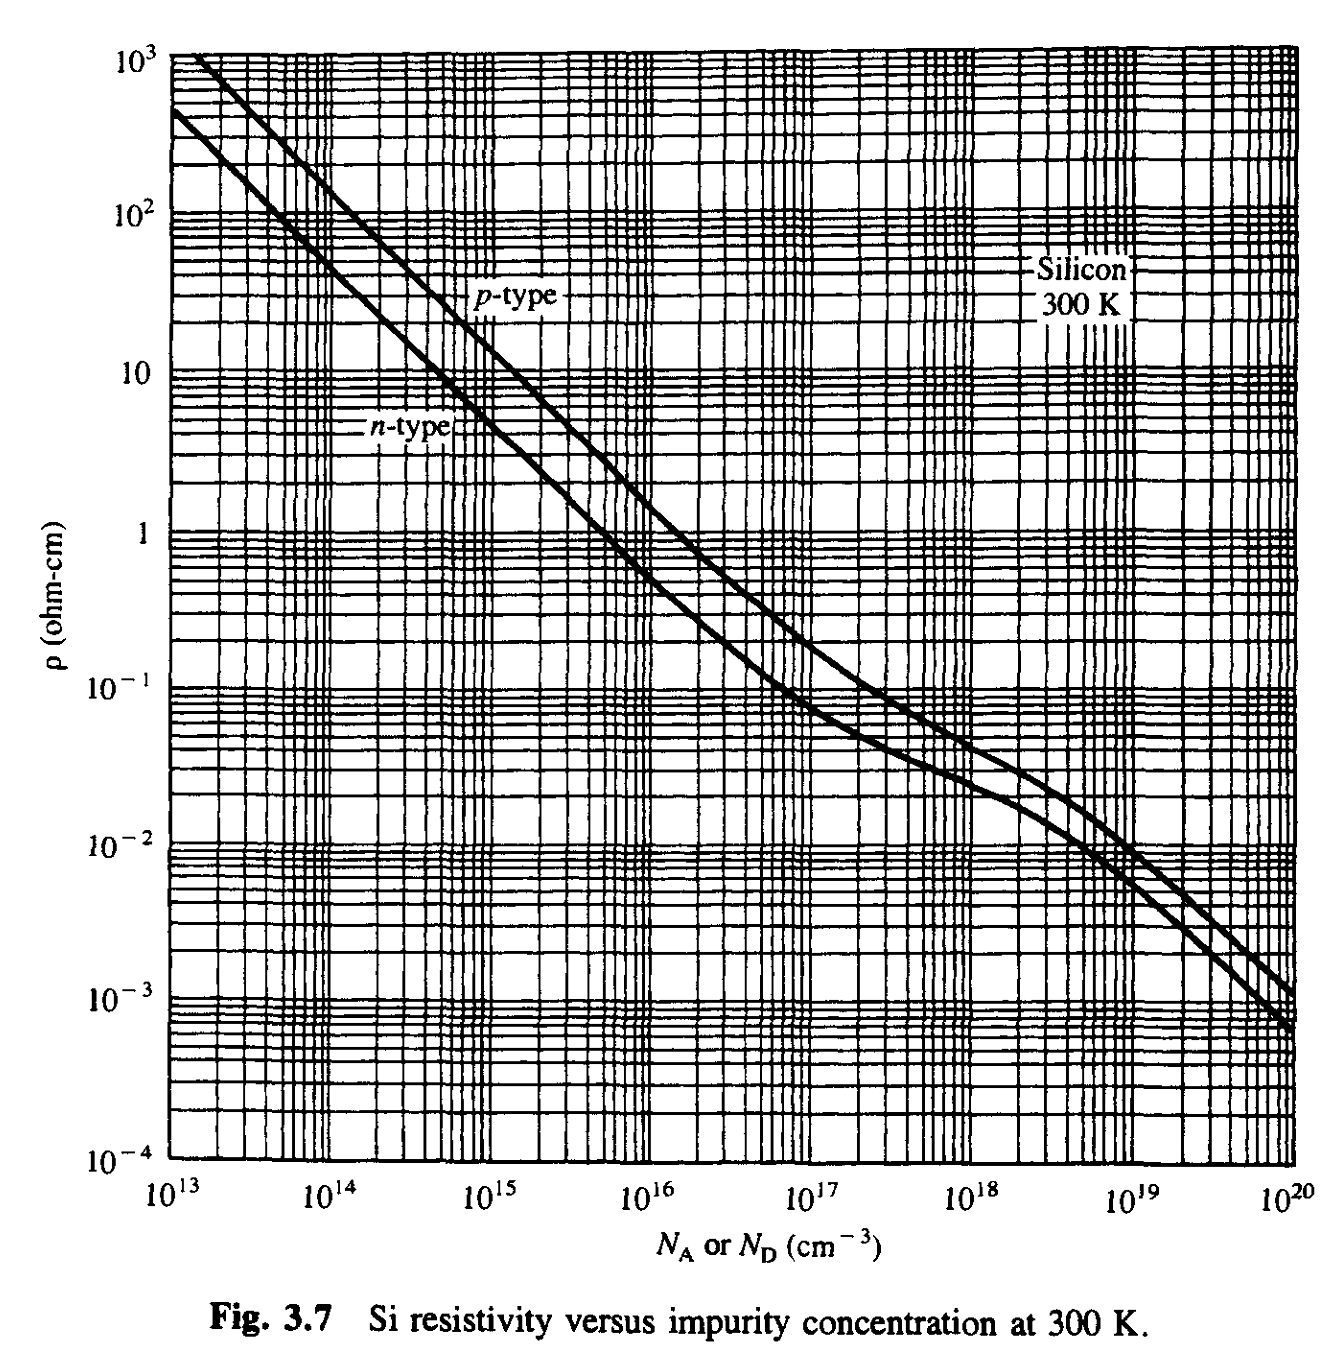
\includegraphics[width=\columnwidth]{VIFigure3-7.png}
            %\captionof{figure}{some caption} % optional
            %\captionof{figure}{some caption} % optional
        \endminipage\medbreak 
        
          \medbreak\noindent\minipage{\columnwidth}
            %\centering % if smaller than \columnwidth
            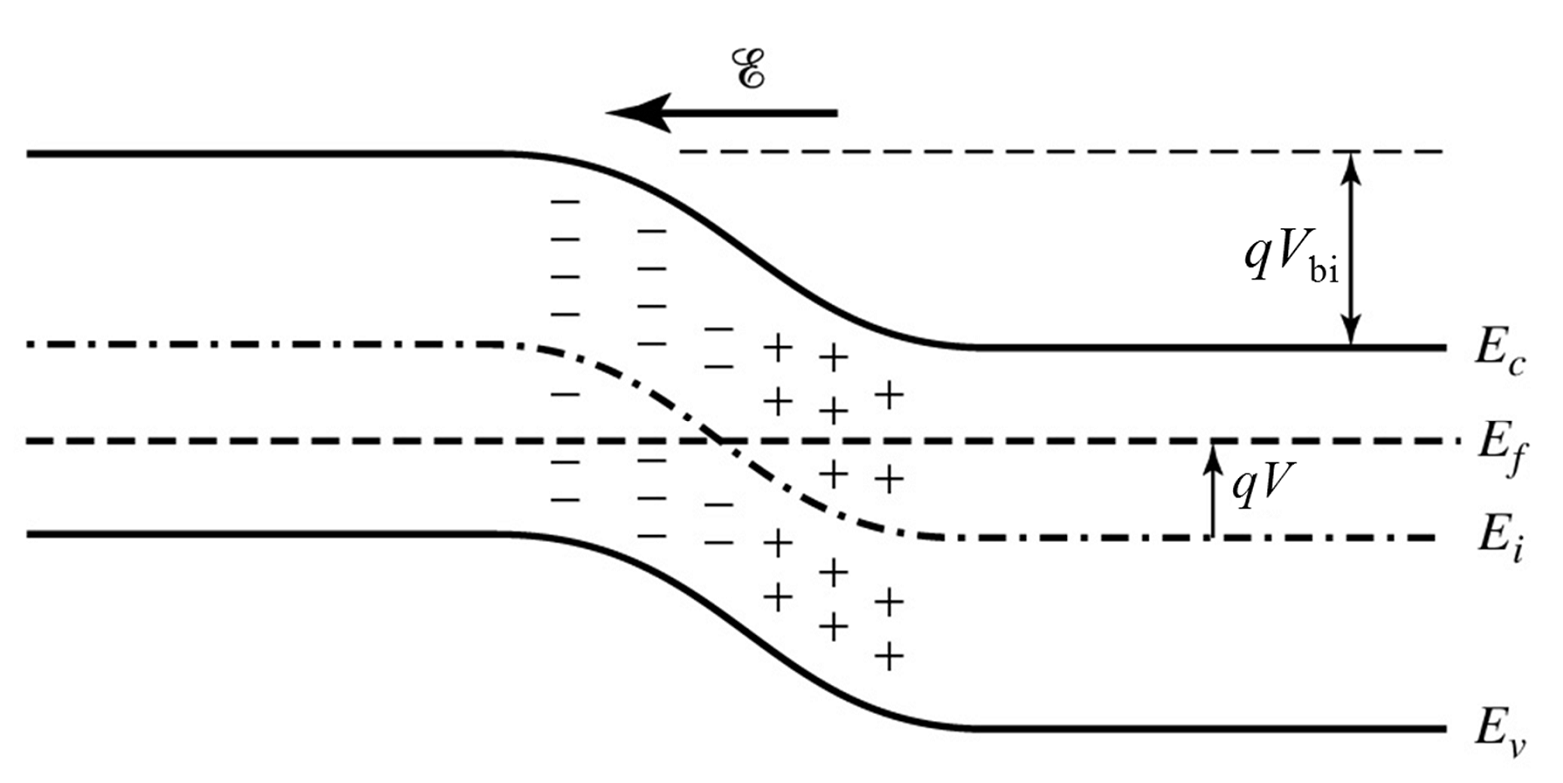
\includegraphics[width=\columnwidth]{LectureNotesIIJunc2.png}
            %\captionof{figure}{some caption} % optional
            %\captionof{figure}{some caption} % optional
        \endminipage\medbreak 
   \end{multicols}
   \newpage
%\paragraph{Useful Images}
\begin{multicols}{2}
  \medbreak\noindent\minipage{\columnwidth}
            %\centering % if smaller than \columnwidth
            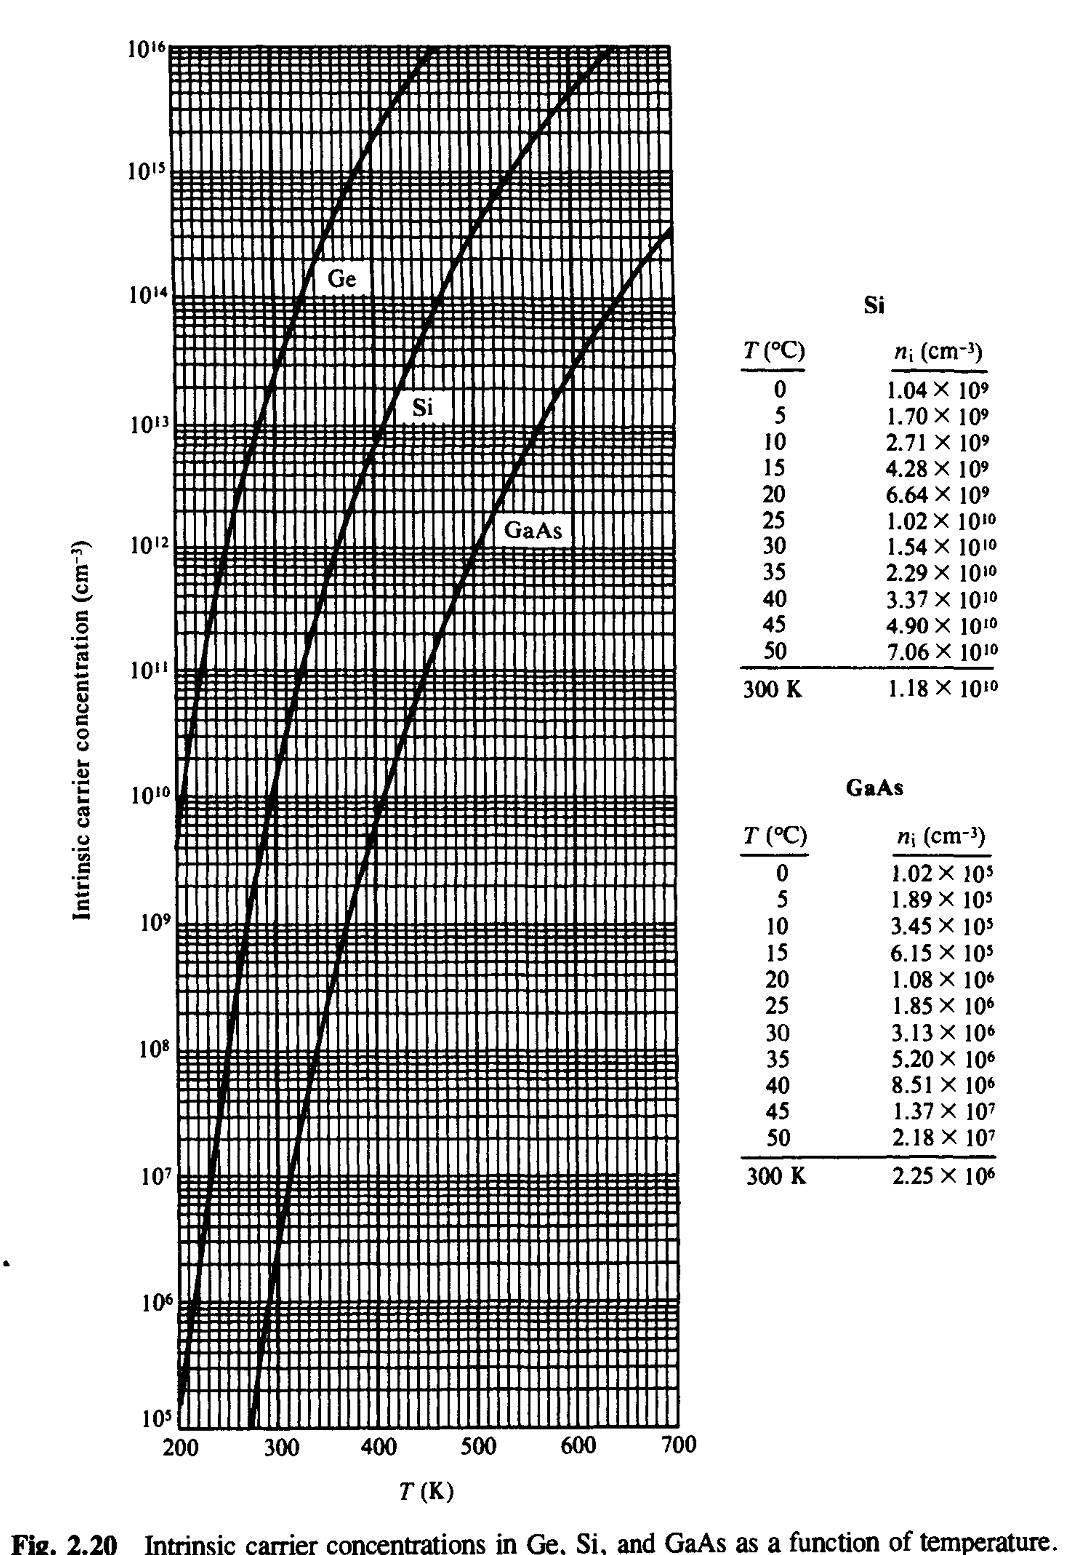
\includegraphics[width=\columnwidth]{V1Figure2-20.png}
            %\captionof{figure}{some caption} % optional
            %\captionof{figure}{some caption} % optional
        \endminipage\medbreak
        
          \medbreak\noindent\minipage{\columnwidth}
            %\centering % if smaller than \columnwidth
            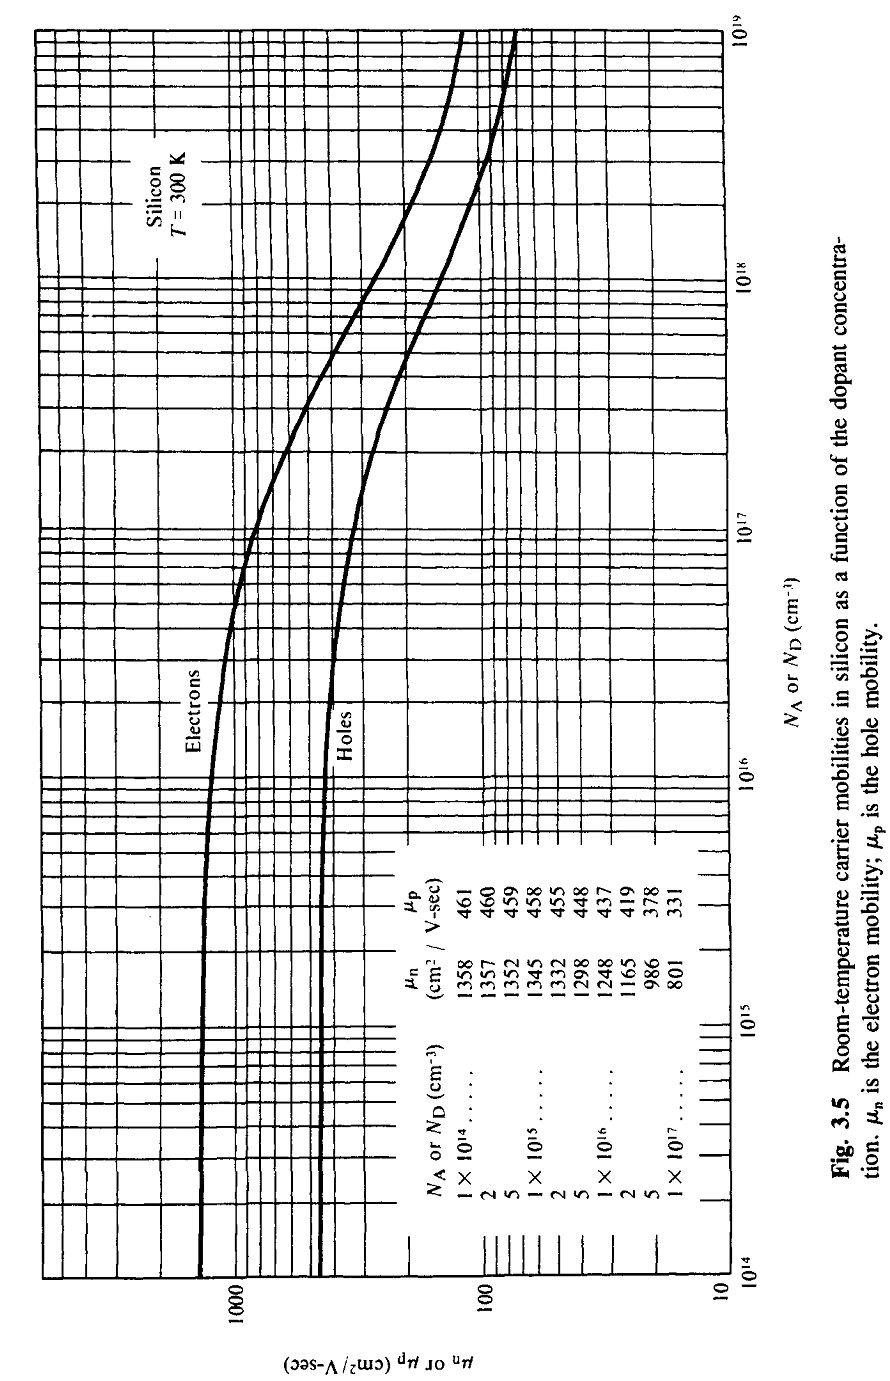
\includegraphics[width=\columnwidth]{V1Figure3-5.png}
            %\captionof{figure}{some caption} % optional
            %\captionof{figure}{some caption} % optional
        \endminipage\medbreak
\end{multicols}